\chapter{Conics}

\section{Dandelin Spheres}
Germinal Pierre Dendelin, a 19th century French-Belgian Professor, discovered this beautiful proof
to demonstrate that any plane that cuts through a right circular cone produces a quadratic curve.
\begin{thm}
  When a plane intersects a right circular cone, the curve produced will either be an ellipse, a parabola or a hyperbola.
\end{thm}
\begin{proof}
  Place a sphere tangent to the intersecting plane $\pi$ and the cone such that it touches the plane at $F$, and the
  cone in a circle $C$ with centre $O$ that lies on a horizontal plane $\epsilon$
  \footnote{Assuming that there exists atleast one such sphere}.\\
  Take an aribtrary point $P$ on the curve $Q$, and extend the line $VP$ from the vertex $V$ of the cone
  to meet $C$ at point $L$. Let $D$ be the point on the intersection on the planes $\pi$ and $\epsilon$ such that
  $PD$ is perpendicular to the line of intersection.(If the planes do not intersect, $Q$ will be a circle)


  \begin{figure}[ht!]
    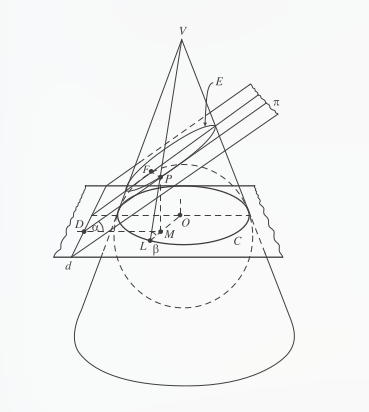
\includegraphics[width=\linewidth]{dandelin.png}
    \caption{When $0<\alpha<\beta<\frac{\pi}{2}$}
  \end{figure}

  Drop a perpendicular $PM$ on $OL$ such that $\triangle PML$ and $\triangle PMD$ are both right angled.
  Denote $\angle PLM$ as $\alpha$, and $\angle PDM$ as $\beta$.\\
  From the triangles  $\triangle PML$ and $\triangle PMD$ 
  
  \begin{eqnarray*}
    \sin{\alpha}&=&\frac{PM}{PD}\\ 
    \quad \textrm{and} \quad \sin{\beta}&=&\frac{PM}{PL}\\
    \quad \textrm{i.e.} \quad \frac{PL}{PD}&=&\frac{\sin{\alpha}}{\sin{\beta}}
  \end{eqnarray*}

  Since $PL$ and $PF$ are both tangents from $P$ to the sphere, $PF=PL$. Therfore,
\[\frac{PF}{PD}=\frac{\sin{\alpha}}{\sin{\beta}}\]
  i.e. $PF=e\cdot PD$, where $e=\sin{\alpha}/\sin{\beta}$\\
  It follows from the focus - directrix definition that $Q$ will be an ellipse if $\alpha<\beta$,
  a parabola if $\alpha=\beta$, or a hyperbola if $\alpha>\beta$.
\end{proof}


\section{Group Laws on Conics}

